\documentclass[conference]{IEEEtran}
\IEEEoverridecommandlockouts
% The preceding line is only needed to identify funding in the first footnote. If that is unneeded, please comment it out.
\usepackage{cite}
\usepackage{amsmath,amssymb,amsfonts}
\usepackage{algorithmic}
\usepackage{graphicx}
\usepackage{textcomp}
\usepackage{xcolor}
\usepackage{enumitem}
\usepackage{stfloats}
\def\BibTeX{{\rm B\kern-.05em{\sc i\kern-.025em b}\kern-.08em
    T\kern-.1667em\lower.7ex\hbox{E}\kern-.125emX}}
\begin{document}

\title{Vision-Based Detection of Protest Behavior in Captive Octopus for Automated Habitat Response}

\author{
\IEEEauthorblockN{
Krishan Mohan Patel\IEEEauthorrefmark{1}\IEEEauthorrefmark{5},
Shivansh Pachnanda\IEEEauthorrefmark{2}\IEEEauthorrefmark{5},
Himanshu Kumar\IEEEauthorrefmark{3},
Amartya Roy\IEEEauthorrefmark{3},\\
Aryavardhan Sharma\IEEEauthorrefmark{3},
Harendra Pal Singh\IEEEauthorrefmark{2},
Harald Burgsteiner\IEEEauthorrefmark{1},
Wolfgang Slany\IEEEauthorrefmark{4}
}

\IEEEauthorblockA{\IEEEauthorrefmark{1}
Institute for Digital Media Education, University of Teacher Education Styria, Graz, Austria
}

\IEEEauthorblockA{\IEEEauthorrefmark{2}
Cluster Innovation Center, University of Delhi, New Delhi, India
}

\IEEEauthorblockA{\IEEEauthorrefmark{3}
Research and Development, Arishna IoT Solutions, Bangalore, India
}

\IEEEauthorblockA{\IEEEauthorrefmark{4}
Institute of Software Engineering and Artificial Intelligence, Graz University of Technology, Graz, Austria
}

\IEEEauthorblockA{\IEEEauthorrefmark{5}
These authors contributed equally (shared first authorship)
}
}
\maketitle


\begin{IEEEkeywords}
Interspecies Communication; Computer Vision; Behavior Detection; Real-time Decision Systems; AI in Marine Biology
\end{IEEEkeywords}

\section{Introduction}
Monitoring behavioral cues in captive marine animals is important for improving welfare and maintaining responsive habitat conditions. In controlled aquarium environments, caretakers often rely on manual observation to identify stress signals or requests for environmental adjustment, which is time-consuming, inconsistent, and requires constant supervision. 

This challenge is greater in species such as octopuses, known for their high intelligence, adaptive behavior, and complex interactions with their surroundings. Their highly flexible body structure, non-rigid movement patterns, camouflage ability, and rapid posture changes make automated visual monitoring particularly difficult. Floating debris, wall reflections, and frequent hiding inside the den further reduce detection reliability in tank-based systems.

We focus on a repeated behavior observed in a captive \emph{O. vulgaris}, from a body weight of 50 g up to 2.8 kg over 7 months, where the animal raises 1--3 limbs upward and moves them frantically to request tank light activation, right after the light was turned off, as shown in Fig.~\ref{fig:behavior_sequence}. The semantic intent of the ``protest" gesture is made clear as the octopus immediately stops the arm gesturing once the light is turned on again. 

In this work, we propose a multi-camera vision-based system to detect this behavior and automatically trigger the lighting system, enabling behavior-driven habitat adaptation and welfare-oriented monitoring. 

\begin{figure*}[!b]
    \centering
    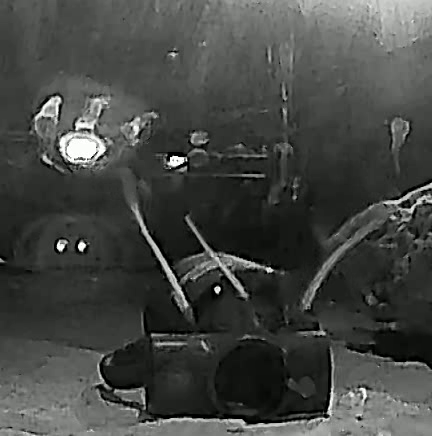
\includegraphics[width=0.16\textwidth]{assets/frames/frame_0039.png}%
    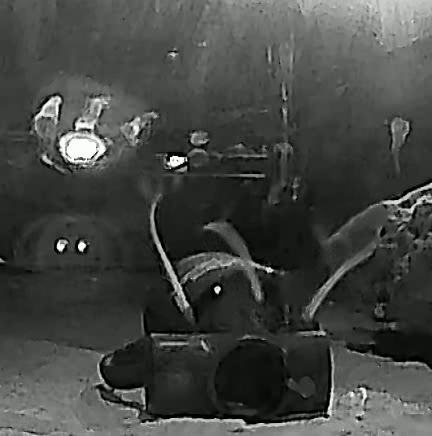
\includegraphics[width=0.16\textwidth]{assets/frames/frame_0042.png}%
    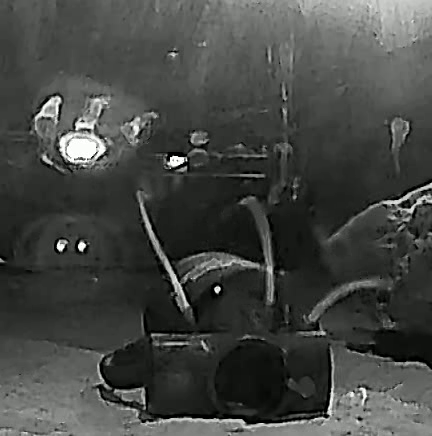
\includegraphics[width=0.16\textwidth]{assets/frames/frame_0045.png}%
    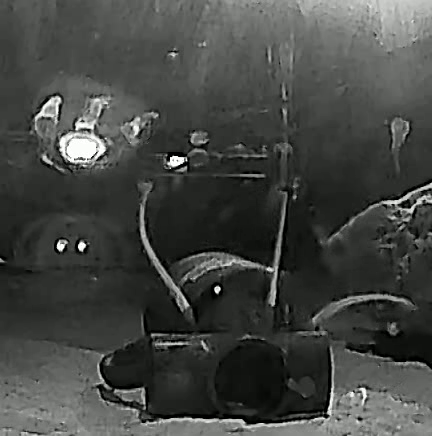
\includegraphics[width=0.16\textwidth]{assets/frames/frame_0048.png}%
    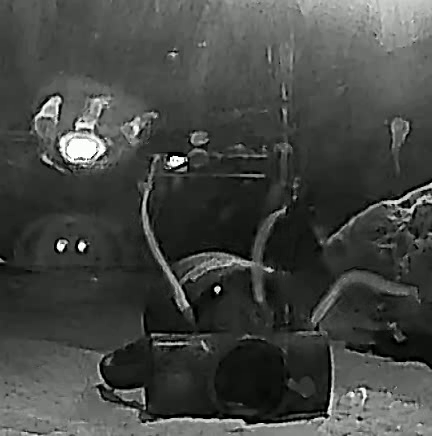
\includegraphics[width=0.16\textwidth]{assets/frames/frame_0051.png}%
    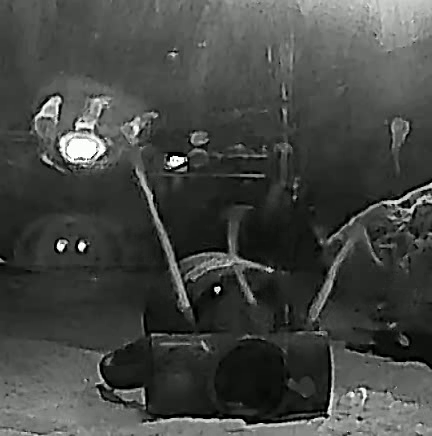
\includegraphics[width=0.16\textwidth]{assets/frames/frame_0054.png}

    \caption{Six sampled frames of octopus (stride of 3) illustrating rapid limb movement near the den region.}

    \label{fig:behavior_sequence}
\end{figure*}

\section{Methodology}

\begin{figure}[htbp]
    \centering
    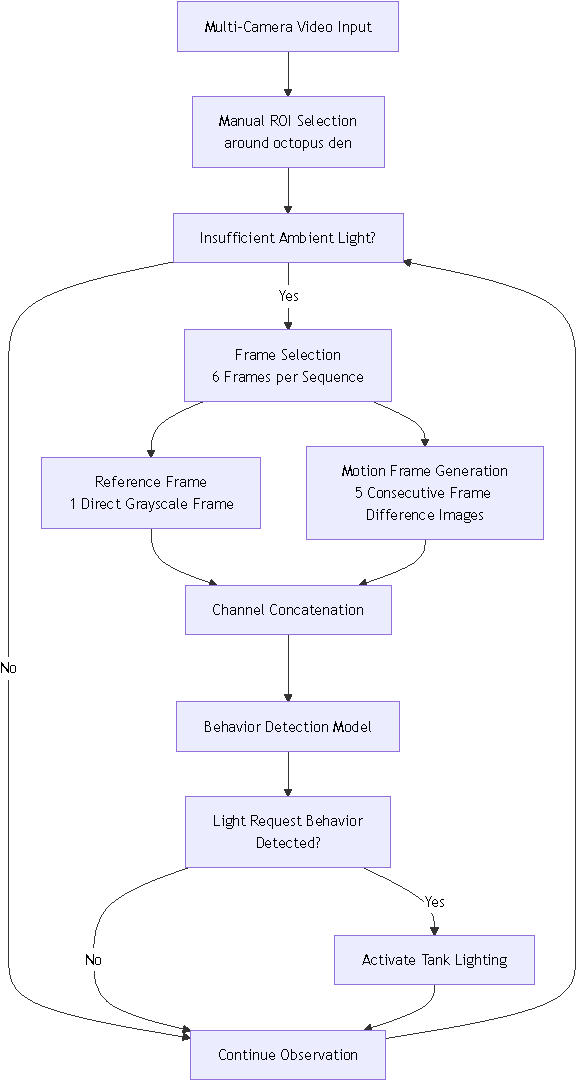
\includegraphics[width=0.36\textwidth]{assets/complete_pipeline_nitty.svg_cropped.pdf}
    \caption{Automated Habitat Response Pipeline}
    \label{fig:model_architecture}
\end{figure}

\begin{itemize}[leftmargin=*, itemsep=2pt, topsep=2pt]

\item \textbf{Setup:} A multi-camera observation system using 6 IP cameras operating at 10 FPS was installed around the captive octopus tank. ANPVIZ 4K 8MP PoE cameras with infrared and colored night vision were used for continuous monitoring. Automated light control was implemented using ANTELA smart WiFi RGB bulbs integrated through Home Assistant via webhook-based automation.

\item \textbf{Data Collection:} A manual Region of Interest (ROI) was selected around the octopus den for each camera. Continuous monitoring has resulted in the collection of $>2$ TB of unannotated 4K video data. Currently, 8 minutes each of positive and negative samples, collected across 36 clips, have been finely annotated, including debris movement, human occlusion, and non-target arm movement, with additional coarse annotations maintained. Ongoing efforts focus on increasing the finely annotated data.

\item \textbf{Frame Selection:} 6-frame sequences with stride 2 were extracted for each sample, consisting of 1 grayscale reference frame and 5 consecutive frame-difference images. These were combined through direct concatenation into a 6-channel input structure.

\item \textbf{Data Augmentation:} Flipping, brightness variation, and random sequence sampling were applied to improve generalization under limited dataset conditions. Random square crops covering approximately 80\% of the selected ROI were also used during training to reduce ROI sensitivity and increase sample variation.

\item \textbf{Behavior Detection Model:} A 1D convolution-based input adapter compresses 6 input channels into 3 before passing to a frozen pretrained backbone network and a lightweight classification head for binary behavior prediction. Pretrained backbones were used to improve robustness and reduce overfitting under limited annotated data conditions.

\item \textbf{Inference and Light Activation:} Inference was performed only under red or low-light conditions, when the octopus has limited visual sensitivity. A rolling 6-frame buffer (1 reference frame and 5 motion-difference frames) was continuously evaluated over 10 inference cycles. Tank lighting was activated only when the average prediction score exceeded a threshold of 0.6, reducing false positives from random noise and non-target motion. See full pipeline in Fig.~\ref{fig:model_architecture}.

\end{itemize}

\section{Preliminary Results}

Preliminary experiments were conducted by comparing multiple pretrained backbone networks for binary classification of the target light-request behavior. See Fig.~\ref{fig:prem_results}.

\begin{figure}[h]
    \centering
    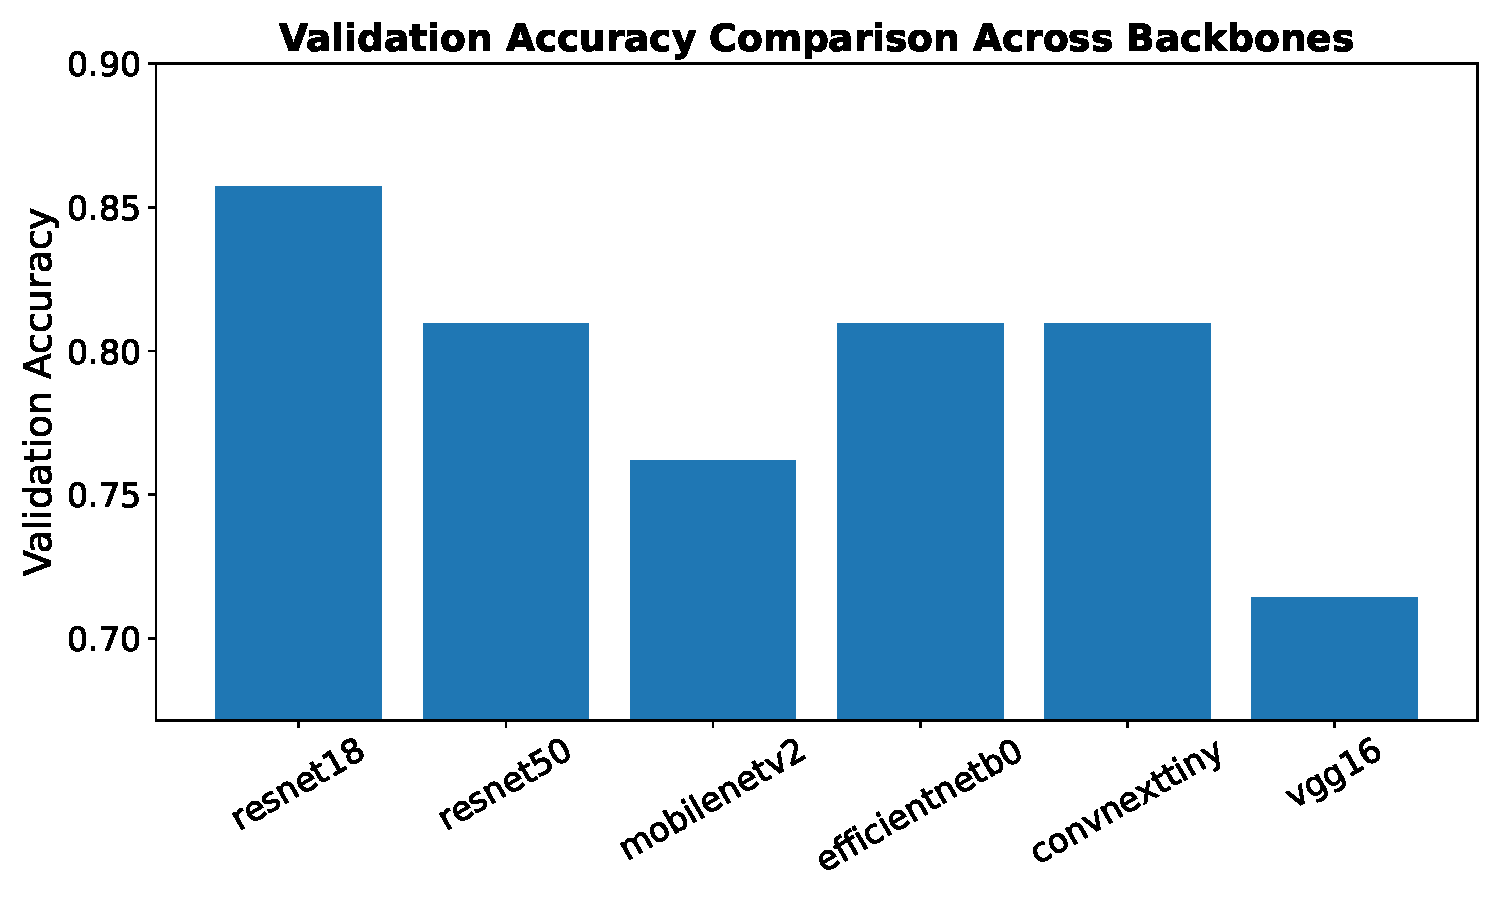
\includegraphics[width=0.5\textwidth]{assets/validation_accuracy_comparison.pdf}
    \caption{Preliminary comparison for binary classification accuracy on val data. Several models show signs of overfitting due to limited finely annotated data; results are subject to change as additional annotations are incorporated.}
    \label{fig:prem_results}
\end{figure}

% 

\section{Relevance to OCEANS Community}

This work contributes to intelligent sensing and real-time response systems for controlled marine habitats, with a primary focus on vision-based behavioral analysis. It aligns with OCEANS themes in imaging and vision systems, as well as real-time autonomous decision-making in marine environments. By enabling behavior-driven environmental control, the framework supports welfare-oriented monitoring and advances responsive habitat management for captive marine species.

Automatic environmental adjustments can improve animal comfort, encourage more natural behavioral expression, and support more reliable observation of repeated patterns. This supports a deeper behavioral understanding and establishes a foundation for future behavior-driven learning systems and intelligent marine habitat management.

\section{Conclusion and Ongoing Work}

The current system serves as an initial proof-of-concept for behavior-driven habitat interaction in controlled marine environments. Ongoing work includes increasing the annotated dataset and developing switch-based interfaces to allow octopus to directly control environmental parameters like tank-lighting, enabling direct communication with its habitat. 

Future work will focus on expanding the framework beyond a single behavior by identifying additional behavioral patterns such as feeding anticipation, stress responses, and interaction-seeking actions. Pose estimation-based behavior detection is also planned to improve recognition accuracy and support the development of a broader welfare-oriented behavior-learning framework for intelligent marine habitat management.

\section*{Ethical Statement and Data Availability} 
The work was conducted in a private aquarium, with only sub-threshold interactions w.r.t. EC directive 2010/63/EU of several caretakers with a single \emph{O. vulgaris} (supplier: Flying Sharks, Portugal). Husbandry and enrichment practices followed best practices for octopus aquariums in compliance with FELASA guidelines. The video data used in the study are available from the last author (W.S.). 

\begin{thebibliography}{00}

\bibitem{b1}
K. Patel, A. Sharma, H. Kumar, P. Kurundodi, H. Burgsteiner, and W. Slany,
``A Novel Framework for Decoding Inter-Species Communication with Octopodes (DISC-O),''
in \textit{OCEANS 2025}, pp. 1--9, Sep. 2025.
doi: 10.23919/OCEANS59106.2025.11244956.

\end{thebibliography}

\end{document}
